\documentclass[12pt,a4paper]{report}
\usepackage[utf8]{inputenc}
\usepackage[english,russian]{babel}
\usepackage{indentfirst}
\usepackage{pdfpages}
\usepackage{titlesec}
\usepackage{listings}
\usepackage{amsmath}

% Вставка картинки
\usepackage{graphicx}
\graphicspath{{schemes/}}
\DeclareGraphicsExtensions{.pdf,.png,.jpg}

\usepackage[tableposition=top,singlelinecheck=false]{caption}

\usepackage[14pt]{extsizes}

\newcommand{\hsp}{\hspace{20pt}}
\titleformat{\chapter}[hang]{\large\bfseries}{\thechapter{. }}{0pt}{\large\bfseries}
\titlelabel{hlabel-formati}
\titlespacing{\chapter}{42pt}{-20pt}{12pt}
\titleformat{\section}[hang]{\large\bfseries}{\thesection{. }}{0pt}{\large\bfseries}
\titlespacing{\section}{42pt}{12pt}{5pt plus 5pt}

% Отступ абзаца
\usepackage{indentfirst}
\setlength{\parindent}{1.5cm}

% Межстрочный интервал
\usepackage{setspace}
\onehalfspacing % интервал 1.5

\usepackage[left=3cm, right=1cm, top=2cm, bottom=2cm]{geometry}

\AtBeginDocument{%
	\renewcommand\contentsname{Содержание}
}

\begin{document}
	% Титульник
	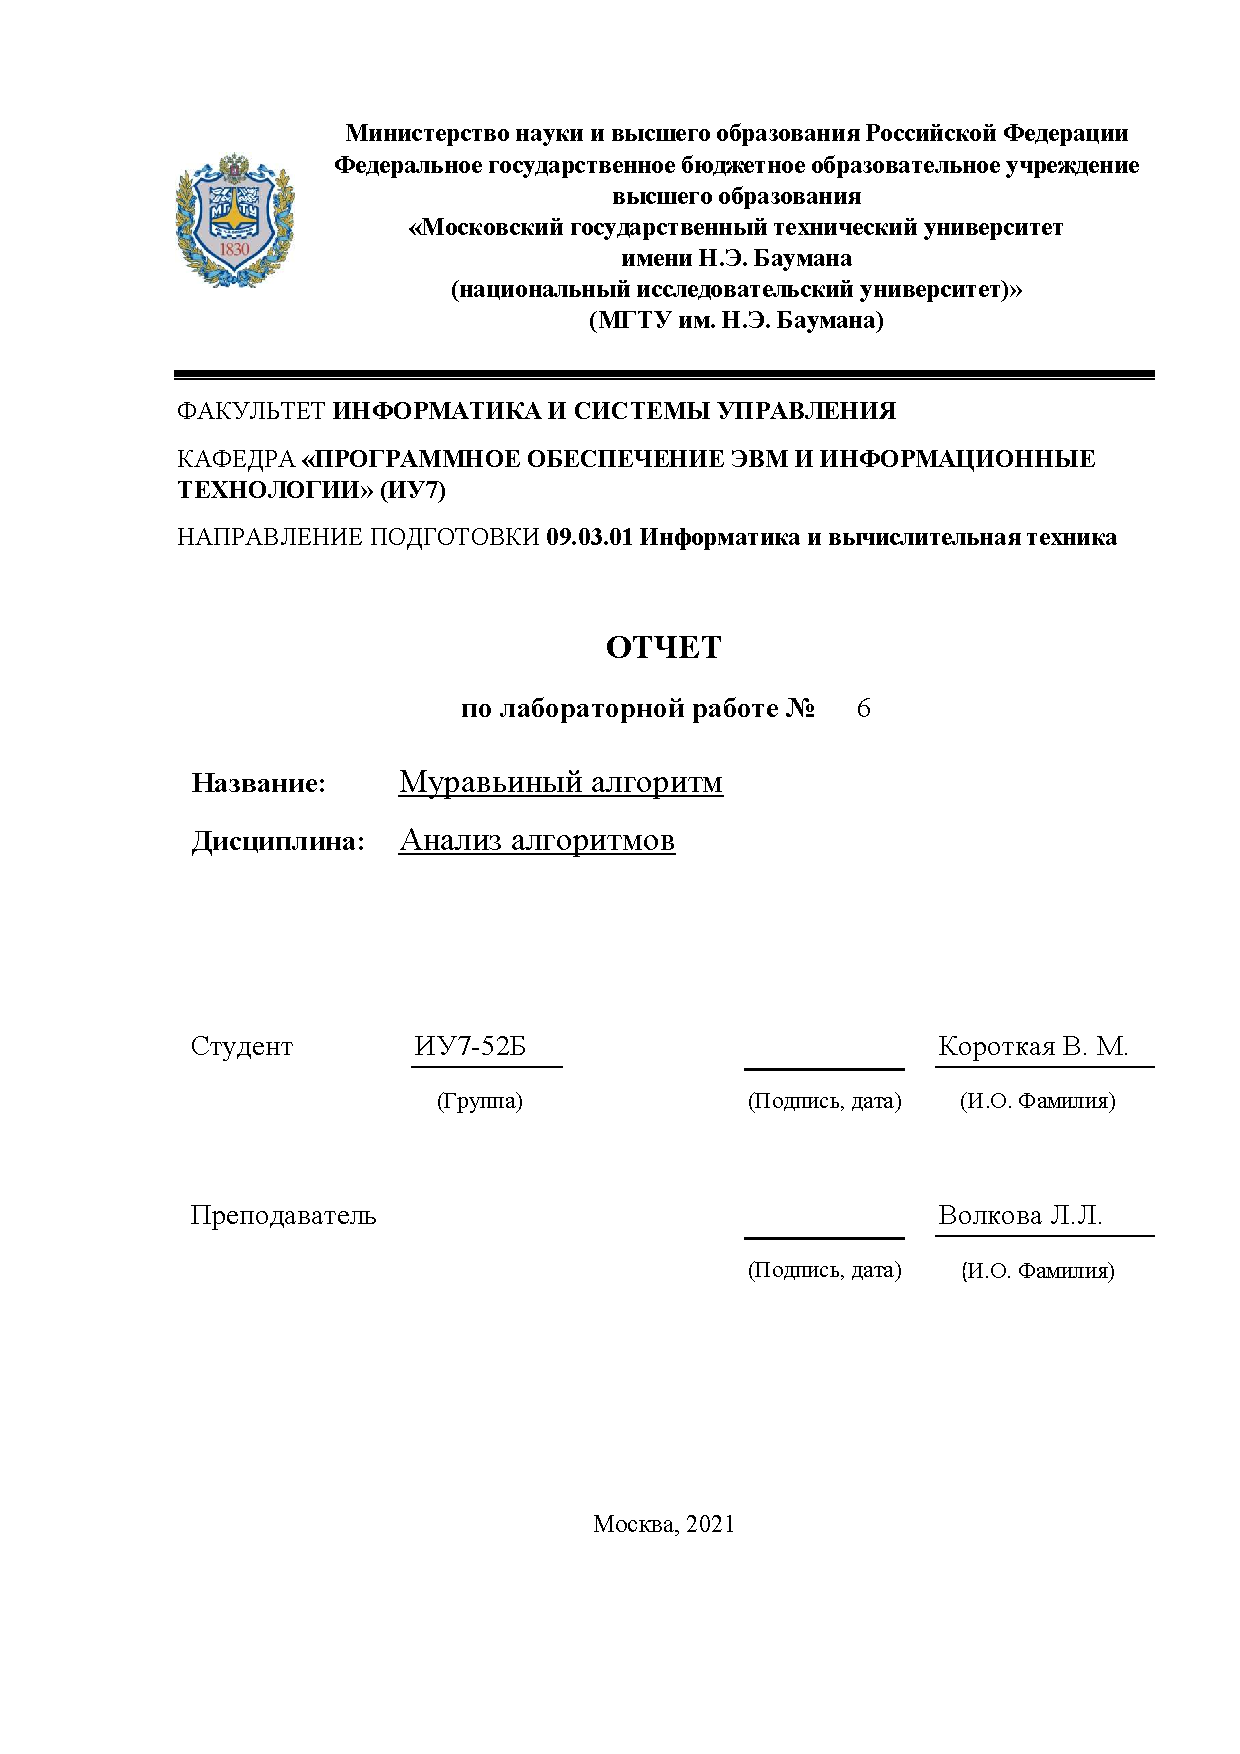
\includepdf[pages=1]{titul.pdf}
	% Оглавление
	\tableofcontents
	
\newpage
\chapter*{Введение}
\addcontentsline{toc}{chapter}{Введение}
	
Муравья нельзя назвать сообразительным. Отдельный муравей не в состоянии принять ни малейшего решения. Дело в том, что он устроен крайне примитивно: все его действия сводятся к элементарным реакциям на окружающую обстановку и своих собратьев. Муравей не способен анализировать, делать выводы и искать решения.

Эти факты, однако, никак не согласуются с успешностью муравьев как вида. Они существуют на планете более 100 миллионов лет, строят огромные жилища, обеспечивают их всем необходимым и даже ведут настоящие войны. В сравнении с полной беспомощностью отдельных особей, достижения муравьев кажутся немыслимыми.

Добиться таких успехов муравьи способны благодаря своей социальности. Они живут только в коллективах – колониях. Все муравьи колонии формируют так называемый роевой интеллект. Особи, составляющие колонию, не должны быть умными: они должны лишь взаимодействовать по определенным – крайне простым – правилам, и тогда колония целиком будет эффективна.

В колонии нет доминирующих особей, нет начальников и подчиненных, нет лидеров, которые раздают указания и координируют действия. Колония является полностью самоорганизующейся. Каждый из муравьев обладает информацией только о локальной обстановке, не один из них не имеет представления обо всей ситуации в целом – только о том, что узнал сам или от своих сородичей, явно или неявно. На неявных взаимодействиях муравьев, называемых стигмергией, основаны механизмы поиска кратчайшего пути от муравейника до источника пищи.

Каждый раз проходя от муравейника до пищи и обратно, муравьи оставляют за собой дорожку феромонов. Другие муравьи, почувствовав такие следы на земле, будут инстинктивно устремляться к нему. Поскольку эти муравьи тоже оставляют за собой дорожки феромонов, то чем больше муравьев проходит по определенному пути, тем более привлекательным он становится для их сородичей. При этом, чем короче путь до источника пищи, тем меньше времени требуется муравьям на него – а следовательно, тем быстрее оставленные на нем следы становятся заметными.

В 1992 году в своей диссертации Марко Дориго (Marco Dorigo) предложил заимствовать описанный природный механизм для решения задач оптимизации. Имитируя поведение колонии муравьев в природе, муравьиные алгоритмы используют многоагентные системы, агенты которых функционируют по крайне простым правилам. Они крайне эффективны при решении сложных комбинаторных задач – таких, например, как задача коммивояжера, первая из решенных с использованием данного типа алгоритмов.


Целью данной работы является изучение и реализация двух алгоритмов:
\begin{itemize}
	\item полный перебор;
	\item муравьиный алгоритм.
\end{itemize}

В рамках выполнения работы необходимо решить следующие задачи:

\begin{itemize}
	\item изучить два, описанных выше алгоритма для решения задачи коммивояжера;
	\item применить изученные знания для реализации двух алгоритмов;
	\item составить схемы алгоритмов;
	\item провести параметризацию муравьиного алгоритма;
	\item провести сравнительный анализ скорости работы реализованных алгоритмов;
	\item выбрать и обосновать выбор языка программирования, для решения поставленной задачи.
\end{itemize}



\newpage
\chapter{Аналитическая часть}


В данном разделе будут рассмортенно формальное описание алгоритмов.

\section{Задача коммивояжера}

В 19-м и 20-м веке по городам ездили коммивояжёры (сейчас их называют «торговые представители»). Они ходили по домам и предлагали людям купить разные товары. Тактика была такой: коммивояжёр приезжал в город, обходил большинство домов и отправлялся в следующий город. Города были небольшими, поэтому обойти всё было вполне реально.

Чем больше городов посетит коммивояжёр, тем больше домов он сможет обойти и больше заработать с продаж.

В задаче коммивояжера рассматривается n городов и матрица
попарных расстояний между ними. Требуется найти такой порядок  посещения  городов,  чтобы  суммарное  пройденное  расстояние было минимальным, каждый город посещался ровно один раз 
и  коммивояжер  вернулся  в  тот  город,  с  которого  начал  свой  маршрут.  Другими  словами,  во  взвешенном  полном  графе  требуется найти \textbf{гамильтонов цикл минимального веса}.



\section{Решение полным перебором}

Эту задачу возможно решить полным перебором т. е. разобрать все возможные варианты и выбрать оптимальный. Но проблема такого решения в том, что с увилечением количества городов, время выполнения будет расти.

Хотя такой подход и гарантирует точное решение задачи, уже при небольшом числе городов решение задачи за допустимое время не возможно.


\section{Решение муравьиным алгоритмом}

В то время как простой метод перебора всех вариантов чрезвычайно
неэффективный при большом количестве городов,
эффективными признаются решения, гарантирующие получение
ответа за время, ограниченное полиномом от размерности задачи.

В основе алгоритма лежит поведение муравьиной колонии -- маркировка более удачных
путей большим количеством феромона.

Каждый муравей хранит в памяти список пройденных им узлов. Этот список называют списком запретов (tabu list) или просто памятью муравья. Выбирая узел для следующего шага, муравей «помнит» об уже пройденных узлах и не рассматривает их в качестве возможных для перехода. На каждом шаге список запретов пополняется новым узлом, а перед новой итерацией алгоритма – то есть перед тем, как муравей вновь проходит путь – он опустошается.

Кроме списка запретов, при выборе узла для перехода муравей руководствуется «привлекательностью» ребер, которые он может пройти. Она зависит, во-первых, от расстояния между узлами (то есть от веса ребра), а во-вторых, от следов феромонов, оставленных на ребре прошедшими по нему ранее муравьями. Естественно, что в отличие от весов ребер, которые являются константными, следы феромонов обновляются на каждой итерации алгоритма: как и в природе, со временем следы испаряются, а проходящие муравьи, напротив, усиливают их.


Вероятность перехода из вершины i в вершину j определяется по формуле 1.1.

\begin{equation}\label{form:way}
	p_{i,j}={\frac {(\tau_{i,j}^{\alpha })(\eta_{i,j}^{\beta })}{\sum (\tau_{i,j}^{\alpha })(\eta_{i,j}^{\beta })}}
\end{equation}

где $ \tau_{i,j} - $ расстояние от города i до j;

$\eta_{i,j} - $количество феромонов на ребре ij;

$\alpha - $ параметр влияния длины пути;

$\beta - $ параметр влияния феромона.

Уровень феромона обновляется в соответствии с формулой \ref{form:eva}


\begin{equation}\label{form:eva}
	\tau_{i,j}=(1-\rho )\tau_{i,j}+\Delta \tau_{i,j},
\end{equation}

где $\rho$ - \text{доля феромона, которая испарится;}

$\tau_{i,j}$ - \text{количество феромона на дуге ij;}

$\Delta \tau_{i,j}$ - количество отложенного феромона, вычисляется по формуле \ref{form:add1}.

\begin{equation}\label{form:add1}
	\Delta \tau_{i,j}= \tau_{i,j}^0 + \tau_{i,j}^1 + ... + \tau_{i,j}^k
\end{equation}

где k - количество муравьев в вершине графа с индексами i и j.


Описание поведения муравьев при выборе пути.

\begin{itemize}
	\item Муравьи имеют собственную «память».
	Поскольку каждый город может быть посещён только один раз, то у каждого муравья есть список уже посещенных городов - список запретов.
	Обозначим через $J_{ik}$ список городов, которые необходимо посетить муравью $k$, находящемуся в городе $i$.
	\item Муравьи обладают «зрением» - видимость есть эвристическое желание посетить город $j$ , если муравей находится в городе $i$.
	Будем считать, что видимость обратно пропорциональна расстоянию между городами.
	\item Муравьи обладают «обонянием» - они могут улавливать след феромона, подтверждающий желание посетить город $j$ из города $i$ на основании опыта других муравьёв.
	Количество феромона на ребре $(i,j)$ в момент времени $t$ обозначим через  $\tau_{i,j} (t)$.
	% \item На этом основании мы можем сформулировать вероятностно - пропорциональное правило, определяющее вероятность перехода $k$-ого муравья из города $i$  в город $j$.
	\item Пройдя ребро $(i,j)$ , муравей откладывает на нём некоторое количество феромона, которое должно быть связано с оптимальностью сделанного выбора.
	Пусть $T _{k} (t)$ есть маршрут, пройденный муравьем $k$ к моменту времени $t$ , $L _{k} (t)$ - длина этого маршрута, а $Q$ - параметр,
	имеющий значение порядка длины оптимального пути. Тогда откладываемое количество феромона может быть задано формулой \ref{form:add}.
	
\end{itemize}



\begin{equation}\label{form:add}
	{\displaystyle \Delta \tau_{i,j}^k={\begin{cases}Q/L_{k}, & {\mbox{если k-ый мурваей прошел по ребру ij;}}\\0,&{\mbox{иначе}}\end{cases}}}
\end{equation}

где Q - количество феромона, переносимого муравьем.

	
\newpage
\section*{Вывод}


В данном разделе были рассмотрены основополагающие материалы,
которые в дальнейшем потребуются при реализации алгоритмов для решения задачи коммивояжера.	
	
	
Входными данными реализуемого ПО являются:

\begin{itemize}
	\item размерность матрицы - натуральное число;
	\item матрица - целочисленная, описывает граф.
\end{itemize}

Выходными данными реализуемого ПО являеться результат алгоритмов т. е.:
\begin{itemize}
	\item последовательность вершин - для полного перебора;
	\item последовательность вершин - для муравьиного алгоритма.
	
\end{itemize}
%Ограничением для реализуемого ПО является - размерность вводимых матриц т. е. длинна строки первой матрицы должна совпадать с длинной колонки второй матрицы.



\chapter{Конструкторская часть}

В данном разделе представлены схемы алгоритмов. Так же будут описаны пользовательские структуры данных, приведены структура ПО и классы эквивалентности для тестирования реализуемого ПО.

\section{Схемы алгоритмов}

На рис. 2.1 показана схема алгоритма полного перебора.

\begin{figure}[ht!]
	\centering{
		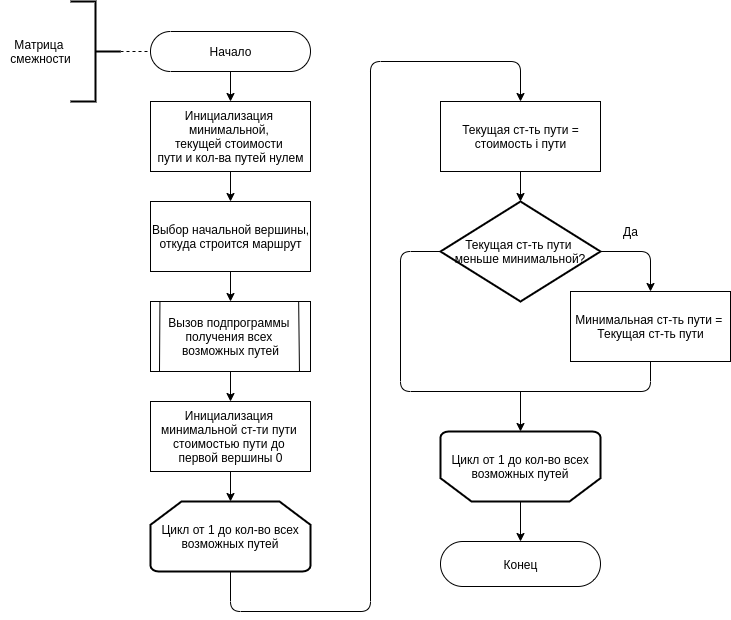
\includegraphics[width=0.9\textwidth]{CompleteBust.png}
		\caption{Схема алгоритма полного перебора}
		\label{ref:d0}}
\end{figure}

\newpage
На рис. 2.2 показана схема муравьиного алгоритма.

\begin{figure}[ht!]
	\centering{
		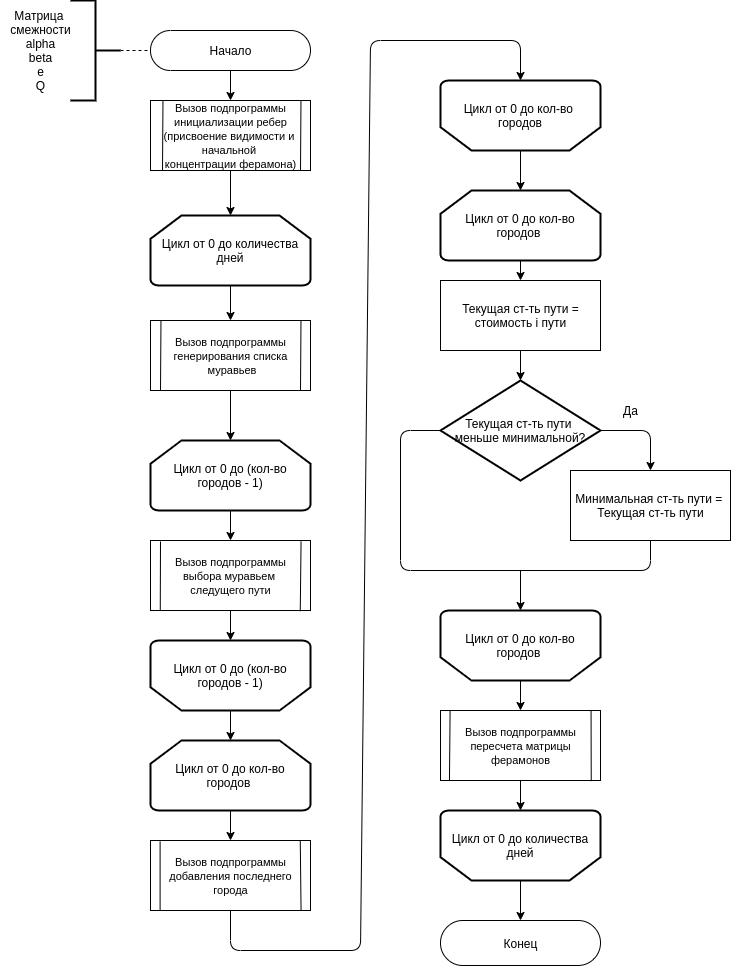
\includegraphics[width=0.9\textwidth]{AntAlgorithm.png}
		\caption{Схема муравьиного алгоритма}
		\label{ref:d1}}
\end{figure}




%\section{Структура ПО}


\newpage
\section{Описание структур данных}

Для реализации данных алгоритмов, введем некоторые типы данных:

\begin{itemize}
	\item ant - тип данных описывающий муравья:
		\begin{itemize}
			\item way - массив посещенных вершин;
			\item route - массив не посищенных вершин.
		\end{itemize}
	\item antColony - тип данных описывающий колонию муравьев:
		\begin{itemize}
			\item graph - граф, описанный матрицей смежности;
			\item ph - матрица, описывающая феромон;
			\item alpha - параметр $ {\alpha }$;
			\item beta - параметр $ {\beta }$;
			\item Q - параметр Q;
			\item p - параметр $ {\rho }$.
		\end{itemize}
\end{itemize}


\section{Классы эквивалентности}

В рамках данной лабороторной можно выделить следующие классы эквивалентности:

\begin{itemize}
	\item входными данными является ациклический ориентированный взвешенный граф;
	\item входными данными является циклический ориентированный взвешенный граф.
\end{itemize}	

Для проверки корректности работы будет проведено функциональное тестирование согласно классам эквивалентности.

\section*{Вывод}

На основе теоритических данных, полученных из аналитического раздела, были построены схемы реализируемых алгоритмов.

Так же, было приведено описание вводимых типов данных.




\newpage
\chapter{Технологическая часть} 

В данном разделе приведены средства реализации, требования к ПО и листинги кода.



\section{Средства реализации}
В качестве языка программирования был выбран с++. Данный язык знаком и предостовляет все необходимые ресурсы.
В качестве среды разработки я использовала Visual Studio Code, т.к. считаю его достаточно удобным и легким.
Visual Studio Code подходит не только для  Windows, но и для Linux, это еще одна причина, по которой я выбрала VS code, т.к. у меня установлена ОС  fedora 34.


%\section{Требования к программному обеспечению}

%Входными данными являются:
%\begin{itemize}
%	\item граф, представленный матрицей смежности;
%\end{itemize}

%На выходе - решение задачи коммивояжера для введенного графа.

\section{Сведенья о модулях программы}

\begin{itemize}
	\item main.cpp - файл, содержащий точку входа в программу;
	\item bruteforce.cpp - файл, содержащий реализацию алгоритма полного перебора;
	\item ant.cpp - файл, содержащий реализацию поведения муравья;
	\item antalgorithm.cpp - файл, содержащий реализацию муравьиного алгоритма;
	\item array.cpp - файл, содержащий реализацию работы с массивом;
	\item matrix.cpp - файл, содержащий реализацию работы с матрицей.
	%\item matrix.cpp - файл, содержащий реализацию алгоритмов умножения матриц.
\end{itemize}   
	
	
\section{Реализация алгоритмов}

В листингах 3.1 - 3.3 приведены реализации алгоритмов на ЯП C++.


%\noindent\textrm{Листинг 3.1: }
%\begin{lstlisting}[frame=single, numbers=left]

%\end{lstlisting}	


\noindent\textrm{Листинг 3.1: Функция релизующая полный перебор.}
\begin{lstlisting}[frame=single, numbers=left]
array get_shortest_path(array cities, int matrix[LEN][LEN])
{
	array result[DEPTH_OF_RECURSION];
	array res_arr;
	
	int min_cost;
	int curr_cost;
	int index = 0;
	
	int routes_count = 0;
	
	del_elem(&cities, 0);
	add_elem(&res_arr, 0);
	get_routes(&cities, &res_arr, result, &routes_count);
	
	min_cost = get_path_cost(result[index], matrix);
	for (int i = 1; i < routes_count; i++)
	{
		curr_cost = get_path_cost(result[i], matrix);
		if (curr_cost < min_cost)
		{
			min_cost = curr_cost;
			index = i;
		}
	}
	
	return result[index];
}
\end{lstlisting}

\noindent\textrm{Листинг 3.2: Функция реализующая муравьинный алгоритм}
\begin{lstlisting}[frame=single, numbers=left]
array ant_algorithm(int matrix[LEN][LEN], int count,
 array cities, int tmax, float p, float alpha, float beta)
{
    int Q = calculate_Q(matrix, count);
    array best_way = copy_arr(cities);
    add_elem(&best_way, get_elem(best_way, 0));
	
    int best_cost = get_path_cost(best_way, matrix);
    int curr_cost = 0;
	
    float matrix_pheromones[LEN][LEN];
    fill_matrix(matrix_pheromones, count, PHEROMONE_MIN);
	
    ant ants[ANTS_MAX_COUNT];
    for (int t = 0; t < tmax; t++)
    {
        generate_ants_array(ants, count);
        for (int i = 0; i < count - 1; i++)
        {
            ants_choose_way(ants, matrix_pheromones, 
                             matrix, count, alpha, beta);
        }
        for (int i = 0; i < count; i++)
            add_elem(&ants[i].way, get_elem(ants[i].way, 0));
        for (int i = 0; i < count; i++)
        {
            curr_cost = get_path_cost(ants[i].way, matrix);
            if (curr_cost < best_cost)
            {
                best_cost = curr_cost;
                best_way = copy_arr(ants[i].way);
            }
        }
        evaporation(matrix_pheromones, count, p);
        add_pheromones(matrix, matrix_pheromones, 
                                     count, Q, ants);
        correct_pheromones(matrix_pheromones, count);
    }
    return best_way;
}
\end{lstlisting}


\noindent\textrm{Листинг 3.3: Функция вычисляющая Q.}
\begin{lstlisting}[frame=single, numbers=left]
int calculate_Q(int matrix[LEN][LEN], int count)
{
    int Q = 0;
	
    for (int i = 0; i < count; i++)
        for (int j = 0; j < i; j++)
            Q += matrix[i][j];
	
    return Q * 2;
}
\end{lstlisting}


\noindent\textrm{Листинг 3.4: Функция реализации добавления ферамона.}
\begin{lstlisting}[frame=single, numbers=left]
void add_pheromones(int matrix[LEN][LEN],  
  float matrix_pheromones[LEN][LEN], int count, int Q,
                             ant ants[ANTS_MAX_COUNT])
{
    int city_first, city_second;
    int curr_cost;
    float delta_tao = 0;
 
    for (int i = 0; i < count; i++)
    {
        curr_cost = get_path_cost(ants[i].way, matrix);
        delta_tao += (float)Q / curr_cost;
    }
	
    for (int i = 0; i < count; i++)
    {
        for (int j = 0; j < ants[i].way.count - 1; j++)
        {
            city_first = ants[i].way.arr[j];
            city_second = ants[i].way.arr[j + 1];
            matrix_pheromones[city_first][city_second] =
             matrix_pheromones[city_first][city_second]
                                             + delta_tao;
            matrix_pheromones[city_second][city_first] =
             matrix_pheromones[city_second][city_first] 
                                             + delta_tao;
        }
    }
}
\end{lstlisting}


%\noindent\textrm{Листинг 3.5: }
%\begin{lstlisting}[frame=single, numbers=left]
%void evaporation(float matrix_pheromones[LEN][LEN],
%                                 int count, float p)
%{
%    float tmp = 1 - p;
%    for (int i = 0; i < count; i++)
%    for (int j = 0; j < i; j++)
%    {
%        matrix_pheromones[i][j] =  
%                        tmp * matrix_pheromones[i][j];
%        matrix_pheromones[j][i] = 
%                        tmp * matrix_pheromones[j][i];
%    }
%}
%\end{lstlisting}


\noindent\textrm{Листинг 3.5: Функция создания муравьев.}
\begin{lstlisting}[frame=single, numbers=left]
void generate_ants_array(ant ants[ANTS_MAX_COUNT],int count)
{
    int elem; 
    for (int i = 0; i < count; i++)
    {
        ants[i].way.count = 0;
        ants[i].route.count = 0;
        elem = rand() % count;
        add_elem(&(ants[i].way), elem);
        for (int j = 0; j < count; j++)
        {
            if (j == elem)
                continue;
            add_elem(&(ants[i].route), j);
        }
    }
}
\end{lstlisting}



\noindent\textrm{Листинг 3.8: Функция реализующая выбор следующего города для муравьем.}
\begin{lstlisting}[frame=single, numbers=left]
void choice_next_city(ant *ants, 
 float matrix_pheromones[LEN][LEN], int matrix[LEN][LEN],
                                  float alpha, float beta)
{
    float numerator = 0;
    float denominator = 0;
    float tao, reverse_cost;
    int cost;
	
    int city_curr = ants->way.arr[ants->way.count - 1];
    for (int i = 0; i < ants->route.count; i++)
    {
        cost = matrix[city_curr][ants->route.arr[i]];
        tao = matrix_pheromones[city_curr][ants->route.arr[i]];
		
        if (!cost)
		    continue;
		
        reverse_cost = 1.0 / cost;
		
        denominator += powf(tao, alpha) + 
                       powf(reverse_cost, beta);
    }
	
    float p_array[LEN] = {0};
    float sum = 0;
    for (int i = 0; i < ants->route.count; i++)
    {
        cost = matrix[city_curr][ants->route.arr[i]];
        tao = matrix_pheromones[city_curr][ants->route.arr[i]];
		
        reverse_cost = 1.0 / cost;
		
        p_array[i] = (powf(tao, alpha) + 
               powf(reverse_cost, beta)) / denominator;
    }

    float x = (float)rand() / RAND_MAX;
    int index = 0;
    while (x >= 0)
    {
        x -= p_array[index];
        index++;
    }
	
    add_elem(&ants->way, get_elem(ants->route, index - 1));
    del_elem(&ants->route, index - 1);
}

\end{lstlisting}


\noindent\textrm{Листинг 3.9: Функция реализующая выбор пути для муравьем}
\begin{lstlisting}[frame=single, numbers=left]
void ants_choose_way(ant ants[ANTS_MAX_COUNT], 
float matrix_pheromones[LEN][LEN], int matrix[LEN][LEN],
 int count, float alpha, float beta)
{
    for (int i = 0; i < count; i++)
    choice_next_city(&ants[i], matrix_pheromones, 
                             matrix, alpha, beta);
}
\end{lstlisting}



%\noindent\textrm{Листинг 3.1: }
%\begin{lstlisting}[frame=single, numbers=left]
	
%\end{lstlisting}






\section{Тестирование}

В таблице \ref{tbl:functional_test} приведены функциональные тесты для алгоритмов сортировки.

\begin{table}[h!]
	\begin{center}
		\caption{Таблица тестов}
		\label{tbl:functional_test}
		\begin{tabular}{c@{\hspace{7mm}}c@{\hspace{7mm}}c@{\hspace{7mm}}c@{\hspace{7mm}}c@{\hspace{7mm}}c@{\hspace{7mm}}c@{\hspace{7mm}}}
			\hline
			Первая матрица & Ожидаемый результат & Жадный & Муравьиный\\ \hline
			\vspace{4mm}
			$\begin{bmatrix}
				0 & 3 & 1 & 6 & 8\\
				3 & 0 & 4 & 1 & 0\\
				1 & 4 & 0 & 5 & 0\\
				6 & 1 & 5 & 6 & 1\\
				8 & 0 & 0 & 1 & 1
			\end{bmatrix}$ &
			15 &
			15 &
			15 \\
			\vspace{2mm}
			\vspace{2mm}
			$\begin{bmatrix}
				0 & 10 & 15 & 20\\
				10 & 0 & 35 & 25 \\
				15 & 35 & 0 & 30 \\
				20 & 25 & 30 & 0
			\end{bmatrix}$ &
			80 &
			80 &
			80 \\
		\end{tabular}
	\end{center}
\end{table}

При проведении функционального тестирования, полученные результаты работы программы совпали с ожидаемыми. Таким образом, функциональное тестирование пройдено успешно.



\section*{Вывод}

В данном разделе были реализованны вышеописанные алгоритмы. Было разработано ПО, удовлетворяющее предьявляемым требованиям. Так же были представлены соответствующие листинги с кодом программы. А так же проведено тестирование разработанного ПО.

\newpage
\chapter{Исследовательская часть} 



В данном разделе будет произведено измерение временных характеристик.
А так же будет выполнена параметризация алгоритма.

\section{Технические характеристики}


Технические характеристики устройства на котором выполнялось исследование:
\begin{itemize}
	\item процессор Intel® Core™ i5-10210U CPU @ 1.60GHz × 8;
	\item память 15.3 GiB;
	\item операционная система Fedora 34 (Workstation Edition) 64-bit.
\end{itemize}

\section{Временные характеристики}

Для сравнения возьмем 8 массивов городов размерностью
$[$3, 4, 5, 6, 7, 8, 9, 10$]$.
Воспользуемся усреднением массового эксперимента.

Результат сравнения муравьиного алгоритма и полного перебора представлен на рис. \ref{ref:time}.

\begin{figure}[ht!]
	\centering{
		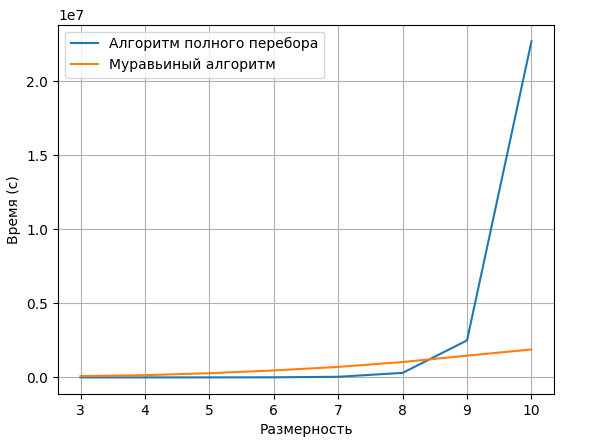
\includegraphics[width=0.7\textwidth]{time1.png}
		\caption{Время работы муравьиного алгоритма и полного перебора}
		\label{ref:time}}
\end{figure}

По результатам эксперимента видно, что время испольнения муравьиного алгоритма
значительно меньше, чем исполнение алгоритма полного перебора.

%\newpage
\section{Параметризация муравьиного алгоритма}

В муравьином алгоритме вычисления производятся на основе настраиваемых параметров.

Рассмотрим матрицу смежностей размерностью $10\times10$ (\ref{table:matrix})

\begin{table}[ht]
	\centering
	\caption{Матрица смежностей}
	\label{table:matrix}
	\begin{tabular}{ | l | l | l | l | l | l | l | l | l | l | l |}
		\hline
		0 & 0    & 1    & 2    & 3    & 4    & 5    & 6    & 7    & 8    & 9    \\ \hline
		0 & 0    & 1790 & 200  & 1900 & 63   & 1659 & 1820 & 1395 & 2382 & 649  \\ \hline
		1 & 1790 & 0    & 1573 & 2435 & 1515 & 714  & 892  & 2193 & 1590 & 1003 \\ \hline
		2 & 200  & 1573 & 0    & 833  & 392  & 2404 & 962  & 902  & 141  & 1123 \\ \hline
		3 & 1900 & 2435 & 833  & 0    & 2283 & 1652 & 2362 & 2262 & 1512 & 2166 \\ \hline
		4 & 63   & 1515 & 392  & 2283 & 0    & 1322 & 290  & 1305 & 2100 & 969  \\ \hline
		5 & 1659 & 714  & 2404 & 1652 & 1322 & 0    & 256  & 78   & 2236 & 2041 \\ \hline
		6 & 1820 & 892  & 962  & 2362 & 290  & 256  & 0    & 1180 & 1547 & 1279 \\ \hline
		7 & 1395 & 2193 & 902  & 2262 & 1305 & 78   & 1180 & 0    & 1640 & 1161 \\ \hline
		8 & 2382 & 1590 & 141  & 1512 & 2100 & 2236 & 1547 & 1640 & 0    & 2212 \\ \hline
		9 & 649  & 1003 & 1123 & 2166 & 969  & 2041 & 1279 & 1161 & 2212 & 0    \\ \hline
	\end{tabular}
\end{table}

%\newpage




\begin{table}[ht!]
	\centering
	\caption{Таблица коэффициентов.(Полную таблицу см. Приложение)}
	\label{table:ref4}
	\begin{tabular}{ | l | l | l | l | l |}
		\hline
		$\alpha$ & $\beta$ & p   & Результат & Разница \\
		\hline
		0        & 1       & 0.7 & 6986      & 0       \\
		0        & 1       & 0.8 & 6986      & 0       \\
		0        & 1       & 0.9 & 6992      & 6       \\
		0        & 1       & 1   & 6986      & 0       \\
		0.1      & 0.9     & 0   & 6986      & 0       \\
		0.1      & 0.9     & 0.7 & 6986      & 0       \\
		0.1      & 0.9     & 0.8 & 6986      & 0       \\
		0.1      & 0.9     & 0.9 & 7165      & 179     \\
		0.1      & 0.9     & 1   & 6986      & 0       \\
		0.2      & 0.8     & 0   & 6986      & 0       \\
		0.3      & 0.7     & 0.1 & 6986      & 0       \\
		0.3      & 0.7     & 0.2 & 7139      & 153     \\
		0.3      & 0.7     & 0.3 & 7139      & 153     \\
		0.3      & 0.7     & 0.4 & 6986      & 0       \\
		0.3      & 0.7     & 0.5 & 6986      & 0       \\
		0.6      & 0.4     & 1   & 6986      & 0       \\
		0.9      & 0.1     & 0.9 & 7376      & 390     \\
			
		1        & 0       & 0.8 & 7874      & 888     \\
		1        & 0       & 0.9 & 7446      & 460     \\
		1        & 0       & 1   & 8119      & 1133    \\
		\hline
	\end{tabular}
\end{table}

\newpage

Параметризация метода решения задачи коммивояжера
на основании муравьиного алгоритма проводилась для матрицы с
элементами в диапозоне [0, 2500].
Количество дней было равно 50.
Полный перебор определил оптимальную длину пути 6986.
Столбец ''результат'' отвечает за результат работы муравьиного алгоритма.
Столбец ''разница'' отвечает за разницу с оптимальной длиной.



\newpage
\section*{Вывод}

На основе проведенной параметризации (таблицы \ref{table:ref1}--\ref{table:ref4}) для матрицы смежности
приведенной в таблице (\ref{table:matrix}) рекомендуется использовать
$(\alpha = 0.5, \beta = 0.5, \rho = \text{любое})$.
При этих параметрах, количество правильно найденных оптимальных путей составило 8 единиц.







\newpage
\chapter*{Заключение}
\addcontentsline{toc}{chapter}{Заключение} 


В данной лабораторной работе были рассмотрены
основополагающие материалы которые в дальнейшем потребовались
при реализации алгоритма полного перебора и муравьиного алгоритма.
Были рассмотрены схемы 
для решения задачи коммивояжера.
Также были разобраны листинги ,
показывающие работу, описанных выше алгоритмов..
Был произведен сравнительный анализ.


В рамках выполнения работы решены следующие задачи:

\begin{itemize}
	\item изучины два, описанных выше алгоритма для решения задачи коммивояжера;
	\item составлины схемы алгоритмов;
	\item проведены параметризацию муравьиного алгоритма;
	\item проведены сравнительный анализ скорости работы реализованных алгоритмов;
\end{itemize}


	
\newpage
\renewcommand\bibname{Список литературы}
\addcontentsline{toc}{chapter}{Список литературы}
\makeatletter % список литературы
\def\@biblabel#1{#1. }
\makeatother
\begin{thebibliography}{2}
	\bibitem{analyse_info} Дж. Макконнел. Анализ алгоритмов. Активный обучающий подход. -- М.: Техносфера, 2017. -- 267с.
	\bibitem{anatyse_info}Основы программирования на языках Си и C++ для начинающих[Электронный ресурс]. Режим доступа: http://cppstudio.com/ (дата обращения 10.10.2021)
	\bibitem{analyse_info}LINUX.ORG.RU - Русскоязычная информация о ОС Linux[Электронный ресурс] Режим доступа://www.linux.org.ru/(дата обращения 25.10.2021)
	\bibitem{analyse_info} Штовба С. Д. Муравьиные алгоритмы, Exponenta Pro. Математика в приложениях. 2004. № 4
	\bibitem{commi} Задача коммивояжера[Электронный ресурс] - режим доступа http://mech.math.msu.su/~shvetz/54/inf/perl-problems/chCommisVoyageur.xhtml
	(дата обращения 25.10.2021)
	
\end{thebibliography}

\newpage
\chapter*{Приложение}

\addcontentsline{toc}{chapter}{Приложение} 

\begin{table}[ht]
	\centering
	\caption{Таблица коэффициентов.Часть 1}
	\label{table:ref1}
	\begin{tabular}{ | l | l | l | l | l |}
		\hline
		$\alpha$ & $\beta$ & p   & Результат & Разница \\
		\hline
		0        & 1       & 0   & 6986      & 0       \\
		0        & 1       & 0.1 & 6986      & 0       \\
		0        & 1       & 0.2 & 6986      & 0       \\
		0        & 1       & 0.3 & 6986      & 0       \\
		0        & 1       & 0.4 & 6986      & 0       \\
		0        & 1       & 0.5 & 6986      & 0       \\
		0        & 1       & 0.6 & 6986      & 0       \\
		0        & 1       & 0.7 & 6986      & 0       \\
		0        & 1       & 0.8 & 6986      & 0       \\
		0        & 1       & 0.9 & 6992      & 6       \\
		0        & 1       & 1   & 6986      & 0       \\
		0.1      & 0.9     & 0   & 6986      & 0       \\
		0.1      & 0.9     & 0.1 & 6992      & 6       \\
		0.1      & 0.9     & 0.2 & 6986      & 0       \\
		0.1      & 0.9     & 0.3 & 6986      & 0       \\
		0.1      & 0.9     & 0.4 & 6986      & 0       \\
		0.1      & 0.9     & 0.5 & 6986      & 0       \\
		0.1      & 0.9     & 0.6 & 6986      & 0       \\
		0.1      & 0.9     & 0.7 & 6986      & 0       \\
		0.1      & 0.9     & 0.8 & 6986      & 0       \\
		0.1      & 0.9     & 0.9 & 7165      & 179     \\
		0.1      & 0.9     & 1   & 6986      & 0       \\
		0.2      & 0.8     & 0   & 6986      & 0       \\
		0.2      & 0.8     & 0.1 & 6986      & 0       \\
		0.2      & 0.8     & 0.2 & 6986      & 0       \\
		0.2      & 0.8     & 0.3 & 6992      & 6       \\
		0.2      & 0.8     & 0.4 & 6992      & 6       \\
		0.2      & 0.8     & 0.5 & 6992      & 6       \\
		0.2      & 0.8     & 0.6 & 6986      & 0       \\
		0.2      & 0.8     & 0.7 & 6992      & 6       \\
		\hline
	\end{tabular}
\end{table}

\begin{table}[ht!]
	\centering
	\caption{Таблица коэффициентов.Часть 2}
	\label{table:ref2}
	\begin{tabular}{ | l | l | l | l | l |}
		\hline
		$\alpha$ & $\beta$ & p   & Результат & Разница \\
		\hline
		
		0.2      & 0.8     & 0.8 & 6986      & 0       \\
		0.2      & 0.8     & 0.9 & 6986      & 0       \\
		0.2      & 0.8     & 1   & 6986      & 0       \\
		0.3      & 0.7     & 0   & 6986      & 0       \\
		0.3      & 0.7     & 0.1 & 6986      & 0       \\
		0.3      & 0.7     & 0.2 & 7139      & 153     \\
		0.3      & 0.7     & 0.3 & 7139      & 153     \\
		0.3      & 0.7     & 0.4 & 6986      & 0       \\
		0.3      & 0.7     & 0.5 & 6986      & 0       \\
		0.3      & 0.7     & 0.6 & 6986      & 0       \\
		0.3      & 0.7     & 0.7 & 6986      & 0       \\
		0.3      & 0.7     & 0.8 & 6992      & 6       \\
		0.3      & 0.7     & 0.9 & 6992      & 6       \\
		0.3      & 0.7     & 1   & 6986      & 0       \\
		0.4      & 0.6     & 0   & 6986      & 0       \\
		0.4      & 0.6     & 0.1 & 6992      & 6       \\
		0.4      & 0.6     & 0.2 & 6986      & 0       \\
		0.4      & 0.6     & 0.3 & 6986      & 0       \\
		0.4      & 0.6     & 0.4 & 6986      & 0       \\
		0.4      & 0.6     & 0.5 & 6992      & 6       \\
		0.4      & 0.6     & 0.6 & 6992      & 6       \\
		0.4      & 0.6     & 0.7 & 6986      & 0       \\
		0.4      & 0.6     & 0.8 & 7139      & 153     \\
		0.4      & 0.6     & 0.9 & 6986      & 0       \\
		0.4      & 0.6     & 1   & 6992      & 6       \\
		0.5      & 0.5     & 0   & 7139      & 153     \\
		0.5      & 0.5     & 0.1 & 6986      & 0       \\
		0.5      & 0.5     & 0.2 & 6986      & 0       \\
		0.5      & 0.5     & 0.3 & 7139      & 153     \\
		0.5      & 0.5     & 0.4 & 6986      & 0       \\
		0.5      & 0.5     & 0.5 & 6986      & 0       \\
		0.5      & 0.5     & 0.6 & 6986      & 0       \\
		0.5      & 0.5     & 0.7 & 6986      & 0       \\
		0.5      & 0.5     & 0.8 & 6986      & 0       \\
		0.5      & 0.5     & 0.9 & 6986      & 0       \\
		0.5      & 0.5     & 1   & 6986      & 0       \\
		0.6      & 0.4     & 0   & 7139      & 153     \\
		0.6      & 0.4     & 0.1 & 6992      & 6       \\
		0.6      & 0.4     & 0.2 & 6986      & 0       \\
		0.6      & 0.4     & 0.3 & 6986      & 0       \\
		0.6      & 0.4     & 0.4 & 7139      & 153     \\
		
		\hline
	\end{tabular}
\end{table}


\begin{table}[ht!]
	\centering
	\caption{Таблица коэффициентов.Часть 3}
	\label{table:ref3}
	\begin{tabular}{ | l | l | l | l | l |}
		\hline
		$\alpha$ & $\beta$ & p   & Результат & Разница \\
		\hline
		
		0.6      & 0.4     & 0.5 & 6992      & 6       \\
		0.6      & 0.4     & 0.6 & 6986      & 0       \\
		0.6      & 0.4     & 0.7 & 6986      & 0       \\
		0.6      & 0.4     & 0.8 & 6986      & 0       \\
		0.6      & 0.4     & 0.9 & 6992      & 6       \\
		0.6      & 0.4     & 1   & 6986      & 0       \\
		0.7      & 0.3     & 0   & 6986      & 0       \\
		0.7      & 0.3     & 0.1 & 6986      & 0       \\
		0.7      & 0.3     & 0.2 & 6986      & 0       \\
		0.7      & 0.3     & 0.3 & 7139      & 153     \\
		0.7      & 0.3     & 0.4 & 7165      & 179     \\
		0.7      & 0.3     & 0.5 & 7139      & 153     \\
		0.7      & 0.3     & 0.6 & 6992      & 6       \\
		0.7      & 0.3     & 0.7 & 6992      & 6       \\
		0.7      & 0.3     & 0.8 & 6986      & 0       \\
		0.7      & 0.3     & 0.9 & 6992      & 6       \\
		0.7      & 0.3     & 1   & 6986      & 0       \\
		0.8      & 0.2     & 0   & 7139      & 153     \\
		0.8      & 0.2     & 0.1 & 7562      & 576     \\
		0.8      & 0.2     & 0.2 & 6992      & 6       \\
		0.9      & 0.1     & 0.2 & 6992      & 6       \\
		0.9      & 0.1     & 0.3 & 6986      & 0       \\
		0.9      & 0.1     & 0.4 & 7139      & 153     \\
		0.9      & 0.1     & 0.5 & 7329      & 343     \\
		0.9      & 0.1     & 0.6 & 7217      & 231     \\
		0.9      & 0.1     & 0.7 & 7139      & 153     \\
		0.9      & 0.1     & 0.8 & 7217      & 231     \\
		0.9      & 0.1     & 0.9 & 7376      & 390     \\
		0.9      & 0.1     & 1   & 6986      & 0       \\
		1        & 0       & 0   & 8531      & 1545    \\
		1        & 0       & 0.1 & 8588      & 1602    \\
		1        & 0       & 0.2 & 6986      & 0       \\
		1        & 0       & 0.3 & 7720      & 734     \\
		1        & 0       & 0.4 & 7554      & 568     \\
		1        & 0       & 0.5 & 6992      & 6       \\
		1        & 0       & 0.6 & 7920      & 934     \\
		1        & 0       & 0.7 & 7217      & 231     \\
		1        & 0       & 0.8 & 7874      & 888     \\
		1        & 0       & 0.9 & 7446      & 460     \\
		1        & 0       & 1   & 8119      & 1133    \\
		\hline
	\end{tabular}
\end{table}

\end{document}	